% "N regularizes model complexity" — a standalone explainer deck
% Decodes the Section-4 claim of Nagler '23 (Statistical Foundations of PFNs).
% Self-contained: no external images. Build with:  make   (tectonic)
\documentclass[aspectratio=169,10pt]{beamer}

\usetheme{metropolis}
\metroset{progressbar=frametitle, numbering=fraction, block=fill}

\usepackage{booktabs}
\usepackage{amsmath,amssymb}
\usepackage{tikz}
\usetikzlibrary{positioning,arrows.meta,fit,backgrounds,calc,decorations.pathreplacing}
\usepackage{pgfplots}
\pgfplotsset{compat=1.18}
\usepackage{xcolor}

% --- palette (matches the main talk) ---------------------------------------
\definecolor{accent}{HTML}{C1121F}
\definecolor{ink}{HTML}{2B2D42}
\definecolor{muted}{HTML}{6C757D}
\definecolor{good}{HTML}{2A9D8F}
\setbeamercolor{frametitle}{bg=ink}
\setbeamercolor{background canvas}{bg=white}
\setbeamercolor{normal text}{fg=ink, bg=white}
\setbeamercolor{progress bar}{fg=accent}
\setbeamercolor{alerted text}{fg=accent}

\newcommand{\hl}[1]{{\color{accent}\textbf{#1}}}
\newcommand{\gd}[1]{{\color{good}\textbf{#1}}}
\newcommand{\mut}[1]{{\color{muted}#1}}
\newcommand{\cit}[1]{{\scriptsize\color{muted}[#1]}}

\title{Why the training size $N$ \emph{regularizes model complexity}}
\subtitle{Decoding one sentence from Section 4 \cit{Nagler '23}}
\author{\underline{Gurmeher} Singh Puri}
\institute{Explainer deck --- frequentist view of PFNs}
\date{}

\begin{document}

\maketitle

% ===========================================================================
\begin{frame}[t]{The sentence we are decoding}

  \onslide<1->{\centering
    From the PFN \emph{approximation} section (\cit{Sec.\ 4}):\par}
  \vspace{0.5em}

  \onslide<1->{\centering
    
\begin{tikzpicture}
      \node[draw=accent, fill=accent!6, rounded corners=3pt, line width=0.9pt,
            inner sep=10pt, text width=0.82\textwidth, align=center, text=ink] {
        ``The training set sizes $N_j$ can thus be seen as a
        \hl{regularizer on model complexity}.''};
    \end{tikzpicture}\par}
  \vspace{0.6em}

  \onslide<2->{\centering Three words to unpack:\par}
  \vspace{0.4em}
  \begin{columns}[T]
    \column{0.32\textwidth}
      \onslide<2->{\centering \hl{$N$} \\ {\footnotesize\mut{the \emph{size} of each simulated training set we show the PFN during pre-training}}\par}
    \column{0.32\textwidth}
      \onslide<3->{\centering \hl{regularizer} \\ {\footnotesize\mut{a knob that limits how \emph{complex} a model is allowed to be (like ridge's $\lambda$, tree depth, bandwidth)}}\par}
    \column{0.32\textwidth}
      \onslide<4->{\centering \hl{complexity} \\ {\footnotesize\mut{how \emph{wiggly} a function the network commits to producing}}\par}
  \end{columns}
  \vspace{0.6em}

  \onslide<4->{\centering {\gd{Claim:}} the \emph{sizes} you train on secretly set the \emph{complexity} of the predictions. Here is why.\par}
\end{frame}

% ===========================================================================
\begin{frame}[t]{Setup: a PFN is trained to copy the PPD, at random sizes}

  \onslide<1->{\centering
    During pre-training we repeatedly: \hl{draw a task}, \hl{simulate a dataset of random size $N_j$}, and
    nudge the net $q_{\hat\theta}$ to match that dataset's PPD.\par}
  \vspace{0.7em}

  \onslide<1->{\centering
  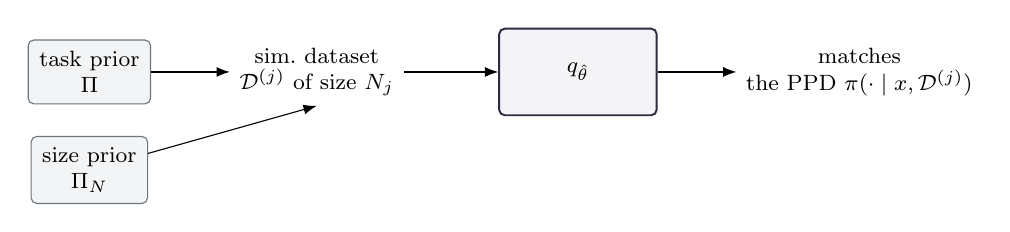
\begin{tikzpicture}[>=Latex, font=\footnotesize, node distance=8mm]
    \node[draw=muted, rounded corners=2pt, fill=muted!8, align=center, inner sep=4pt] (prior)
         {task prior\\ $\Pi$};
    \node[draw=muted, rounded corners=2pt, fill=muted!8, align=center, inner sep=4pt, below=4mm of prior] (sizes)
         {size prior\\ $\Pi_N$};
    \node[align=center, right=10mm of prior] (data)
         {sim.\ dataset\\ $\mathcal{D}^{(j)}$ of size $N_j$};
    \node[draw=ink, fill=ink!5, rounded corners=2pt, line width=0.7pt, align=center,
          minimum width=20mm, minimum height=11mm, right=12mm of data] (net) {$q_{\hat\theta}$};
    \node[align=center, right=10mm of net] (out) {matches\\ the PPD $\pi(\cdot\mid x,\mathcal{D}^{(j)})$};
    \draw[->] (prior) -- (data);
    \draw[->] (sizes) -- ($(data.south)+(0,-0.0)$);
    \draw[->] (data) -- (net);
    \draw[->] (net) -- (out);
  \end{tikzpicture}}
  \vspace{0.7em}

  \onslide<2->{\centering
    For \hl{TabPFN}: $\Pi_N=$ \emph{uniform on} $\{1,\dots,1023\}$. \;\mut{\footnotesize (why so small? next-to-last slide.)}\par}
  \vspace{0.3em}

  \onslide<3->{\centering
    Key question: as the size $N$ changes, does the \emph{ideal} network change too?\par}
\end{frame}

% ===========================================================================
\begin{frame}[t]{Fact 1 --- the target's complexity \emph{grows} with $n$}

  \onslide<1->{\centering
    The thing we copy is the PPD $\pi(y\mid x,\mathcal{D}_n)$. How wiggly it is depends on $n$:\par}
  \vspace{0.8em}

  \onslide<1->{\centering
  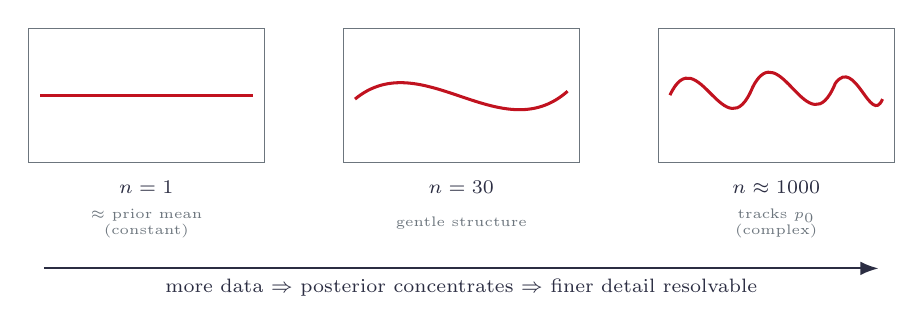
\begin{tikzpicture}[>=Latex]
    % panel 1: n=1, constant
    \begin{scope}
      \draw[muted, line width=0.4pt] (0,0) rectangle (3,1.7);
      \draw[accent, line width=1.1pt] (0.15,0.85) -- (2.85,0.85);
      \node[ink, font=\scriptsize] at (1.5,-0.32) {$n=1$};
      \node[muted, font=\tiny, align=center] at (1.5,-0.78) {$\approx$ prior mean\\ (constant)};
    \end{scope}
    % panel 2: n moderate, one bump
    \begin{scope}[shift={(4,0)}]
      \draw[muted, line width=0.4pt] (0,0) rectangle (3,1.7);
      \draw[accent, line width=1.1pt] (0.15,0.8) .. controls (1.0,1.5) and (2.0,0.15) .. (2.85,0.9);
      \node[ink, font=\scriptsize] at (1.5,-0.32) {$n=30$};
      \node[muted, font=\tiny, align=center] at (1.5,-0.78) {gentle structure};
    \end{scope}
    % panel 3: n large, wiggly
    \begin{scope}[shift={(8,0)}]
      \draw[muted, line width=0.4pt] (0,0) rectangle (3,1.7);
      \draw[accent, line width=1.1pt]
        (0.15,0.85) .. controls (0.5,1.6) and (0.85,0.1) .. (1.2,0.95)
                    .. controls (1.55,1.65) and (1.9,0.15) .. (2.25,1.0)
                    .. controls (2.5,1.35) and (2.7,0.45) .. (2.85,0.8);
      \node[ink, font=\scriptsize] at (1.5,-0.32) {$n\approx1000$};
      \node[muted, font=\tiny, align=center] at (1.5,-0.78) {tracks $p_0$\\ (complex)};
    \end{scope}
    % arrow underneath
    \draw[->, ink, line width=0.8pt] (0.2,-1.35) -- (10.8,-1.35)
        node[midway, below, font=\scriptsize] {more data $\Rightarrow$ posterior concentrates $\Rightarrow$ finer detail resolvable};
  \end{tikzpicture}}
  \vspace{1.0em}

  \onslide<2->{\centering
    {\footnotesize\mut{$n=1$: one point can't reveal structure, so the PPD is essentially the average prior model --- nearly flat.}}\par}
\end{frame}

% ===========================================================================
\begin{frame}[t]{Fact 2 --- so the \emph{ideal parameters} follow the size}

  \onslide<1->{\centering
    Define the KL-optimal parameter \emph{for a fixed size} $n$:
    \;$\displaystyle \theta^*_n=\arg\max_{\theta}\ \mathbb{E}_{\Pi}\bigl[\log q_{\theta}(Y\mid X,\mathcal{D}_n)\bigr]$.\par}
  \vspace{0.6em}

  \onslide<1->{\centering
  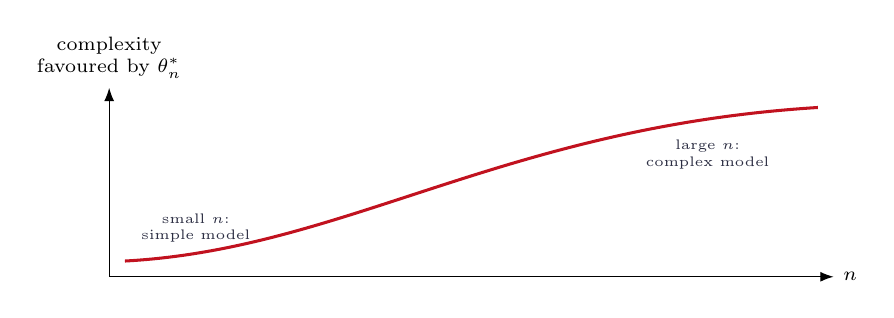
\begin{tikzpicture}[>=Latex, font=\footnotesize]
    \draw[->] (0,0) -- (9.2,0) node[right, font=\scriptsize]{$n$};
    \draw[->] (0,0) -- (0,2.4) node[above, font=\scriptsize, align=center]{complexity\\ favoured by $\theta^*_n$};
    \draw[accent, line width=1.1pt] (0.2,0.2) .. controls (3.0,0.35) and (5.0,1.9) .. (9.0,2.15);
    \node[ink, align=center, font=\tiny] at (1.1,0.62) {small $n$:\\ simple model};
    \node[ink, align=center, font=\tiny] at (7.6,1.55) {large $n$:\\ complex model};
  \end{tikzpicture}}
  \vspace{0.5em}

  \onslide<2->{\centering
    The target $\pi(\cdot\mid x,\mathcal{D}_n)$ changes with $n$ $\;\Rightarrow\;$ its best approximator $\theta^*_n$ does too:
    \hl{bigger sets justify (and demand) more complexity}.\par}
  \vspace{0.4em}

  \onslide<3->{\centering
    But training optimises an \emph{average} over $N_j\sim\Pi_N$:
    \;$\hat\theta$ blends the $\theta^*_{N_j}$. \;{\gd{So $\Pi_N$ sets the \emph{average} complexity.}}\par}
\end{frame}

% ===========================================================================
\begin{frame}[t]{The analogy that makes it click: \#points caps the fit}

  \onslide<1->{\centering
    Fit a curve to data. The \emph{number of points} alone tells you how complex a fit is sensible.\par}
  \vspace{0.4em}

  \begin{columns}[T]
    \column{0.5\textwidth}
      \onslide<1->{\centering \textbf{2 points}\\[4pt]
      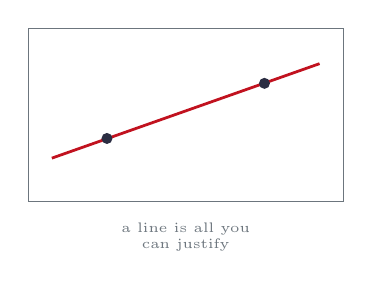
\begin{tikzpicture}[>=Latex]
        \draw[muted, line width=0.4pt] (0,0) rectangle (4,2.2);
        \draw[accent, line width=1.0pt] (0.3,0.55) -- (3.7,1.75);
        \fill[ink] (1.0,0.8) circle(0.07);
        \fill[ink] (3.0,1.5) circle(0.07);
        \node[muted, font=\tiny, align=center] at (2.0,-0.45) {a line is all you\\ can justify};
      \end{tikzpicture}}
    \column{0.5\textwidth}
      \onslide<2->{\centering \textbf{many points}\\[4pt]
      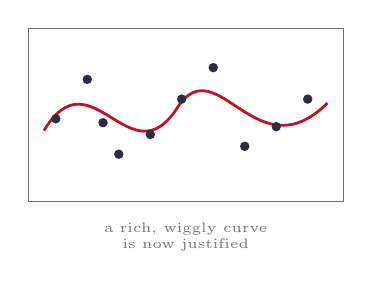
\begin{tikzpicture}[>=Latex]
        \draw[muted, line width=0.4pt] (0,0) rectangle (4,2.2);
        \draw[accent, line width=1.0pt]
          (0.2,0.9) .. controls (0.8,1.9) and (1.3,0.25) .. (1.9,1.2)
                    .. controls (2.4,1.95) and (2.9,0.35) .. (3.8,1.25);
        \foreach \p in {(0.35,1.05),(0.75,1.55),(1.15,0.6),(1.55,0.85),(1.95,1.3),
                        (2.35,1.7),(2.75,0.7),(3.15,0.95),(3.55,1.3),(0.95,1.0)}
          \fill[ink] \p circle(0.06);
        \node[muted, font=\tiny, align=center] at (2.0,-0.45) {a rich, wiggly curve\\ is now justified};
      \end{tikzpicture}}
  \end{columns}
  \vspace{0.3em}

  \onslide<3->{\centering
    A degree-9 polynomial through 2 points is nonsense (\mut{over-fitting}). The PPD, being Bayes-optimal,
    \hl{automatically} stays simple when data is scarce.\par}
\end{frame}

% ===========================================================================
\begin{frame}[t]{Therefore: $\Pi_N$ is a complexity dial = a regularizer}

  \onslide<1->{\centering
    Choosing where $\Pi_N$ puts its mass is choosing how complex the network's predictions become.\par}
  \vspace{0.8em}

  \onslide<1->{\centering
  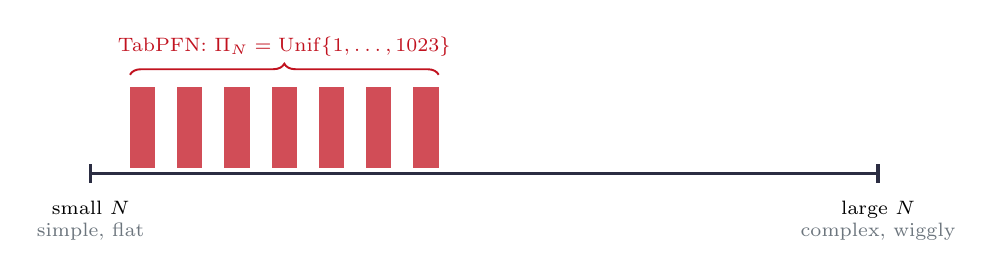
\begin{tikzpicture}[>=Latex, font=\footnotesize]
    % the dial axis
    \draw[line width=1.2pt, ink] (0,0) -- (10,0);
    \foreach \x in {0,10} \draw[ink, line width=1.2pt] (\x,-0.12)--(\x,0.12);
    \node[align=center, font=\scriptsize] at (0,-0.6) {small $N$\\ \mut{simple, flat}};
    \node[align=center, font=\scriptsize] at (10,-0.6) {large $N$\\ \mut{complex, wiggly}};
    % uniform{1..1023} mass shown as bars over the lower-left stretch
    \onslide<2->{%
      \foreach \x in {0.5,1.1,1.7,2.3,2.9,3.5,4.1}
        \fill[accent!75] (\x,0.06) rectangle (\x+0.32,1.1);
      \draw[decorate, decoration={brace, amplitude=4pt}, accent, line width=0.7pt]
        (0.5,1.25) -- (4.42,1.25)
        node[midway, above=3pt, text=accent, font=\scriptsize] {TabPFN: $\Pi_N=\mathrm{Unif}\{1,\dots,1023\}$};
    }
  \end{tikzpicture}}
  \vspace{0.9em}

  \onslide<3->{\centering
    Same role as a classic regularizer --- it trades off complexity:\par}
  \vspace{0.2em}
  \onslide<3->{\centering
    \begin{tabular}{ccc}
      \hl{ridge $\lambda$} & \hl{tree depth} & \hl{kernel bandwidth} \\
      \multicolumn{3}{c}{\footnotesize\mut{$\cdots$ and now: \gd{the size prior $\Pi_N$}}}
    \end{tabular}\par}
\end{frame}

% ===========================================================================
\begin{frame}[t]{One subtlety --- don't misstate this in Q\&A}

  \begin{columns}[T]
    \column{0.5\textwidth}
      \onslide<1->{\begin{block}{Ordinary regularizer}
        \begin{itemize}\setlength\itemsep{4pt}
          \item adds a \hl{penalty on the parameters} (e.g.\ $+\lambda\|\theta\|^2$)
          \item acts \emph{directly} on the model
        \end{itemize}
      \end{block}}
    \column{0.5\textwidth}
      \onslide<2->{\begin{block}{Here ($\Pi_N$)}
        \begin{itemize}\setlength\itemsep{4pt}
          \item \hl{no penalty on $\theta$ at all}
          \item you reshape the \emph{training distribution} so the \emph{optimal target} is simpler/more complex
          \item regularizes \hl{indirectly}
        \end{itemize}
      \end{block}}
  \end{columns}
  \vspace{0.8em}

  \onslide<3->{\centering
    The \emph{effect} on realised complexity is the same --- that is why he calls it a regularizer ---\\
    but the \emph{mechanism} is ``control the data sizes,'' not ``penalize the weights.''\par}
\end{frame}

% ===========================================================================
\begin{frame}[t]{Why it matters --- this loads the spring for the puzzle}

  \onslide<1->{\centering
    TabPFN caps $\Pi_N$ at ${\approx}1000$ \hl{purely for compute}: a transformer costs $\mathcal{O}(N^2)$.\par}
  \vspace{0.6em}

  \onslide<1->{\centering
  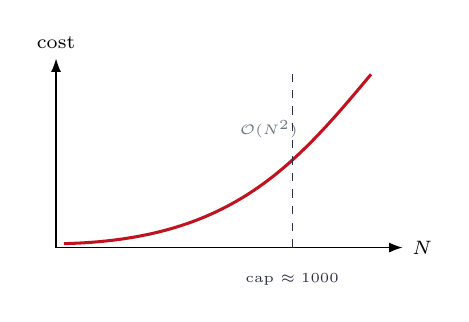
\begin{tikzpicture}[>=Latex, font=\footnotesize]
    \draw[->] (0,0) -- (4.4,0) node[right, font=\scriptsize]{$N$};
    \draw[->] (0,0) -- (0,2.4) node[above, font=\scriptsize]{cost};
    \draw[accent, line width=1.1pt] (0.1,0.05) .. controls (2.2,0.1) and (3.0,1.0) .. (4.0,2.2);
    \node[muted, font=\tiny] at (2.7,1.5) {$\mathcal{O}(N^2)$};
    \draw[dashed, ink] (3.0,0) -- (3.0,2.2);
    \node[ink, font=\tiny, align=center] at (3.0,-0.4) {cap $\approx1000$};
  \end{tikzpicture}}
  \vspace{0.7em}

  \onslide<2->{\centering
    So the net is \hl{regularized to be no more complex than ${\le}1000$-point targets require}.\par}
  \vspace{0.4em}

  \onslide<3->{\centering
    {\gd{The puzzle, sharpened:}} a network whose complexity was tuned for ${\le}1000$ points
    \emph{still improves} when fed far more.\\[2pt]
    {\footnotesize\mut{$\Rightarrow$ Section 5 (frequentist view) answers \emph{how}: mostly by \hl{shrinking variance}, not by inventing new complexity.}}\par}
\end{frame}

% ===========================================================================
\begin{frame}[standout]
  $N$ small $\Rightarrow$ simple target $\Rightarrow$ simple net.\\[6pt]
  The \emph{size prior} $\Pi_N$ is the complexity dial.
\end{frame}

\end{document}
